%!TEX root = ../report.tex

% 
% Overview
% 

\section{Overview} % (fold)
\label{sec:overview}


This section will provide an overview of this topic, where we explain some procedural modeling techniques that we aim to support, with some examples of application for the architects and designers. We will also introduce in Section~\ref{sub:graphic_tools} some technology that is used in the solution .  Section~\ref{sec:related_work} will explore related work. Section~\ref{sec:objectives} will address the objectives for this thesis work. Section~\ref{sec:architecture} will describe the architecture of the proposed solution. Section~\ref{sec:evaluation} will explain how this solution will be evaluated and section~\ref{sec:conclusions} will conclude this work.

\subsection{Procedural Modeling} % (fold)
\label{sub:procedural_modeling}

\emph{Procedural Modeling} is the algorithmic generation of content instead of the usual manual creation of content. This can be applied in almost all forms of content, but is mostly used in the generation of graphic content, such as textures, geometry and animations, in which is included generative design. Procedural generation is also used for the generation of sound, with procedurally generated music and synthetic speech.

The key property of procedural generation is that it describes the data entities, such as textures, geometry, or sounds, in terms of a sequence of instructions rather than as a static block of data \cite{Kelly}. This allows the production of big volumes of detailed, high quality, graphic content without the costs, both in time and money, of manual content creation. Since it is based on procedures, it provides parametric control. Users can introduce in their programs as many useful parameters as they want, which allows them, for instance, to have different results from just one implementation by just changing some control values.


\subsection{Procedural Modeling Techniques} % (fold)
\label{sub:procedural_modeling_techniques}

In the following sections are explained some procedural modeling techniques. These techniques are applied to the generation of various types of forms procedurally.

% subsection procedural_modeling_techniques (end)

%!TEX root = ../../report.tex

\subsection{Fractals} % (fold)
\label{ssub:fractals}


A fractal is defined in \cite{Ebert2002} as ``a geometrically complex object, the complexity of which arises through the repetition of a given form over a range of scales''.
This concept is observed in some forms that exist in nature. From trees, mountains, coastlines to the network of neurons on a human cortex can be seen as examples of fractals. Natural shapes tend to be irregular and fragmented and exhibit a complexity incomparable to regular geometry \cite{mandelbrot1984fractal}.
In \cite{Ebert2002} is proposed to think of fractals as a new form of symmetry, \emph{Dilation Symmetry}, which is when an object is invariant over a change of scale. This invariance migth be only qualitatively and not exact. For instance, a river network exhibit dilation symmetry if \textit{zooming in} in some part looks the same as the whole image. As this example, many others show dilated symmetry. As clouds, tree branches and some vegetables as shown in Figure~\ref{fig:NFractals}. These examples are fractals.

\begin{figure}
        \centering
        \begin{subfigure}[b]{0.4\textwidth}
                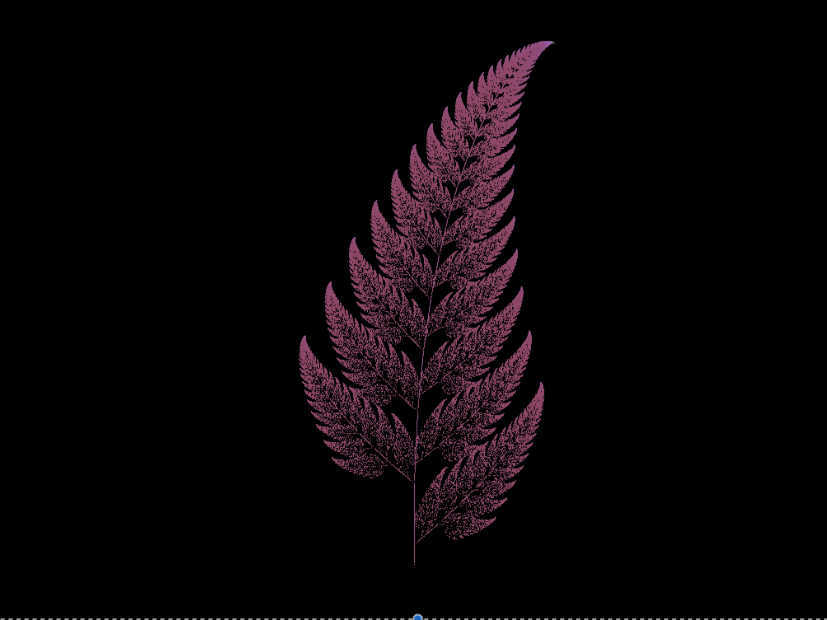
\includegraphics[width=\textwidth]{img/Theory/Fractals/Leaf.png}
                \label{fig:Fleaf}
        \end{subfigure}%
        ~ %add desired spacing between images, e. g. ~, \quad, \qquad, \hfill etc.
          %(or a blank line to force the subfigure onto a new line)
        \begin{subfigure}[b]{0.4\textwidth}
                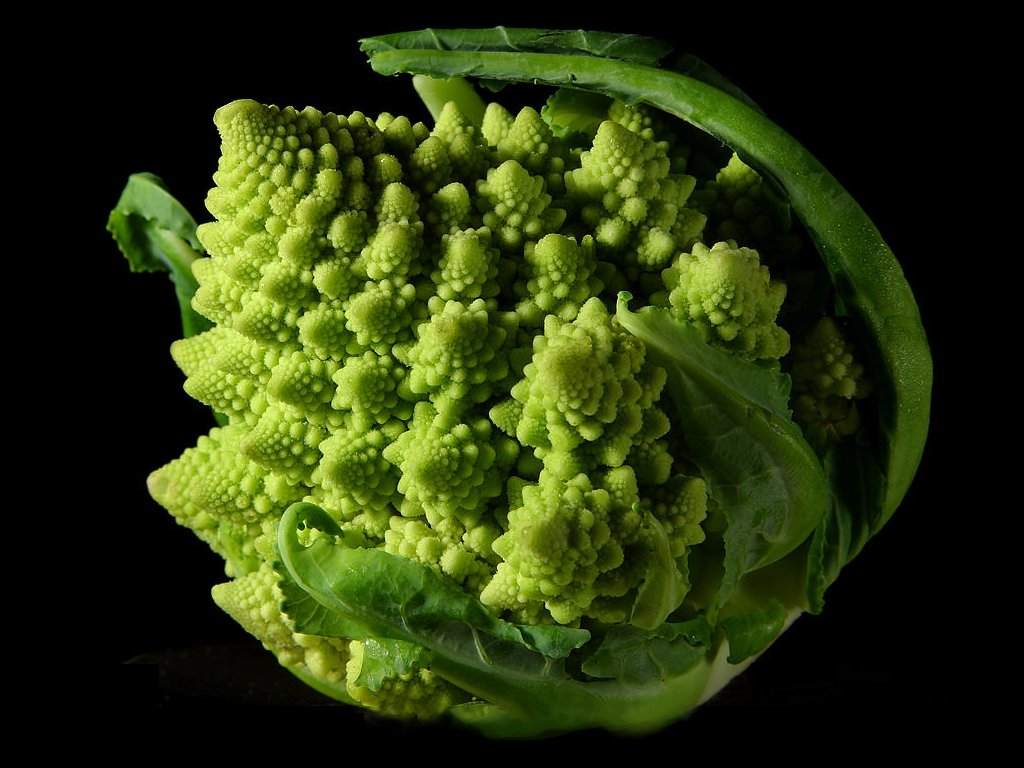
\includegraphics[width=\textwidth]{img/Theory/Fractals/Fractal_Broccoli.jpg}
                \label{fig:Fbrocoli}
        \end{subfigure}
        \caption{Fractals in Nature}\label{fig:NFractals}
\end{figure}


This idea was applied in maths with the evolution of a new area in this science called fractal mathematics. The objective of this field is to describe this very complex shapes with really simple rules as repeating a substitution pattern. 

\begin{figure}[htbp]
	\centering
	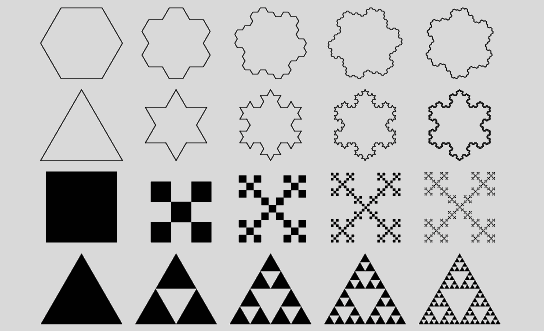
\includegraphics[width=0.7\textwidth]{img/Theory/Fractals/Fractal1_1000.png}
	\caption{Geometric Fractals}
	\label{fig:GFractals}
\end{figure}

In the Figure~\ref{fig:GFractals} there are four examples of Geometric Fractals, with the first five iterations of each one. All of them are built by the substitution of a part of the image by another one. 

The example of the second row is known as the Koch snowflake. In this example, at each iteration, all the line segments are replaced by four segments with 1/3 of the size of the original one with the two in the middle being placed in a angle forming a equilateral triangle with the original line that is removed.

It's clear that the detail that is presented in each iteration increases as the scale changes. To try to mesure this evolution there is the concept of \emph{Fractal Dimension} in which the detail in a pattern changes in comparison with the scale in which it is measured.

As stated before, the world is visualy very complex, so when synthetizing worlds, ``\emph{complexity} equals \emph{work}''\cite{Ebert2002}. This work can be done by the programer/artist or by a computer. Some cases are not easy to model procedurally. This is not the case of the fractals, as being defined as a simple mathematical function, it's relatively easy to implement a procedure to model fractals. 

This techique is used to model many natural forms that present fractal properties. Mountains, as an instance, are usually modeled using of fractals. Other natural forms that present fractal properties are trees, river systems, ligthning or vascular systems in living beings.




% subsection fractals (end)


%!TEX root = ../../report.tex

\subsubsection{Cellular Automaton} % (fold)
\label{sub:cellular_automaton}

A cellular Automaton is a model of a system of cells within a grid with a given shape, each of this cells can be on one of a finite set of states. It evolves during a finite amount of time steps with a set of simple rules according to each state of the neighboring cells.
The neighborhood of the cell can be defined in many different ways, the most common is the use of the adjacent cells. 

This models have various applications, such as modeling of nature aspects (Figure~\ref{fig:CArule30shell}), textures, and as inspiration to architecture (Figure~\ref{fig:CAarchitecture}).

\begin{figure}
        \centering
        \begin{subfigure}[b]{0.5\textwidth}
                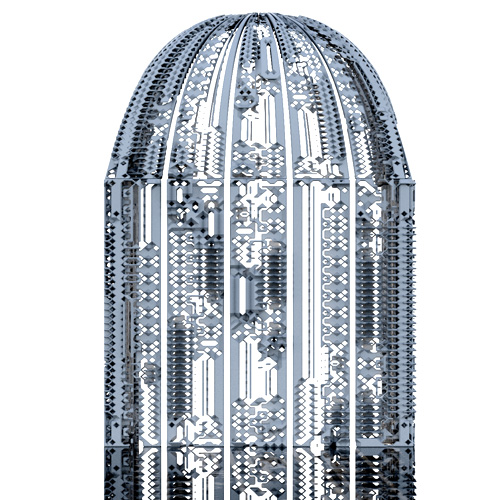
\includegraphics[width=\textwidth]{img/Theory/Cellular_A/dome1.jpg}
                \caption{}
  %              \label{fig:CAdome}
        \end{subfigure}%
        %~ %add desired spacing between images, e. g. ~, \quad, \qquad, \hfill etc.
          %(or a blank line to force the subfigure onto a new line)
          ~~
        \begin{subfigure}[b]{0.5\textwidth}
                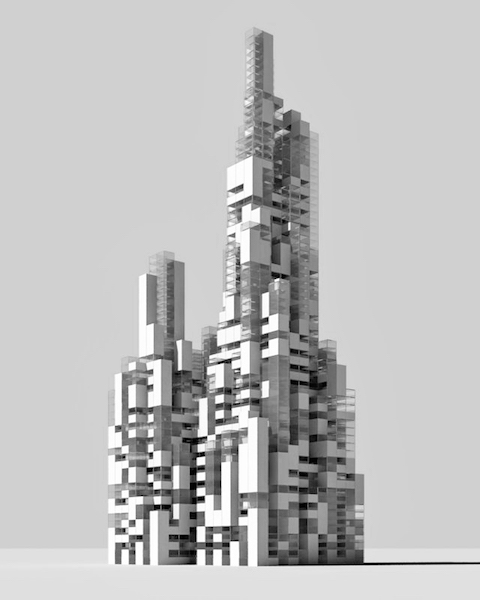
\includegraphics[width=\textwidth]{img/Theory/Cellular_A/main1.jpg}
                \caption{}
   %             \label{fig:CArule30}
        \end{subfigure}
        \caption{Examples of cellular automata applied in architecture}
        \label{fig:CAarchitecture}
\end{figure}

The case where each cell have two possible states and the next generation state depends only on the previous state of the cell and the two immediate neighbors is called an \emph{elementary cellular automaton}. In this case we have $2^3 = 8$ possible patterns for a neighborhood and $2^8 = 256$ sets of possible different rules. This rules are referred by their \emph{Wolfram code} \cite{CellularAutWOLFRAM}. 

A common initial state for this elementary cellular automata is a random line. But to be able to compare the results between rules and get clean results another option is to start with a line with zeros except the middle cell that is initialized with the value one. Applying this second option and the set of rules in Figure~\ref{fig:CArule} (the rule 30), we get the pattern in the Figure~\ref{fig:resultCA} that represents the evolution of a cellular automaton over a few generations.

\begin{figure}[htbp]
	\centering
	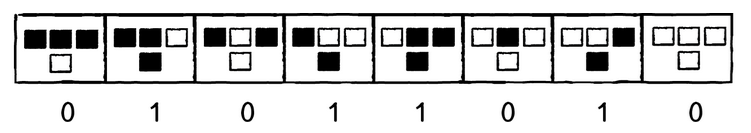
\includegraphics[width=0.85\textwidth]{img/Theory/Cellular_A/Rules.png}
	\caption{Example Production Rules\cite{Shiffman2012}}
	\label{fig:CArule}
\end{figure}



\begin{figure}[H]
    \centering
    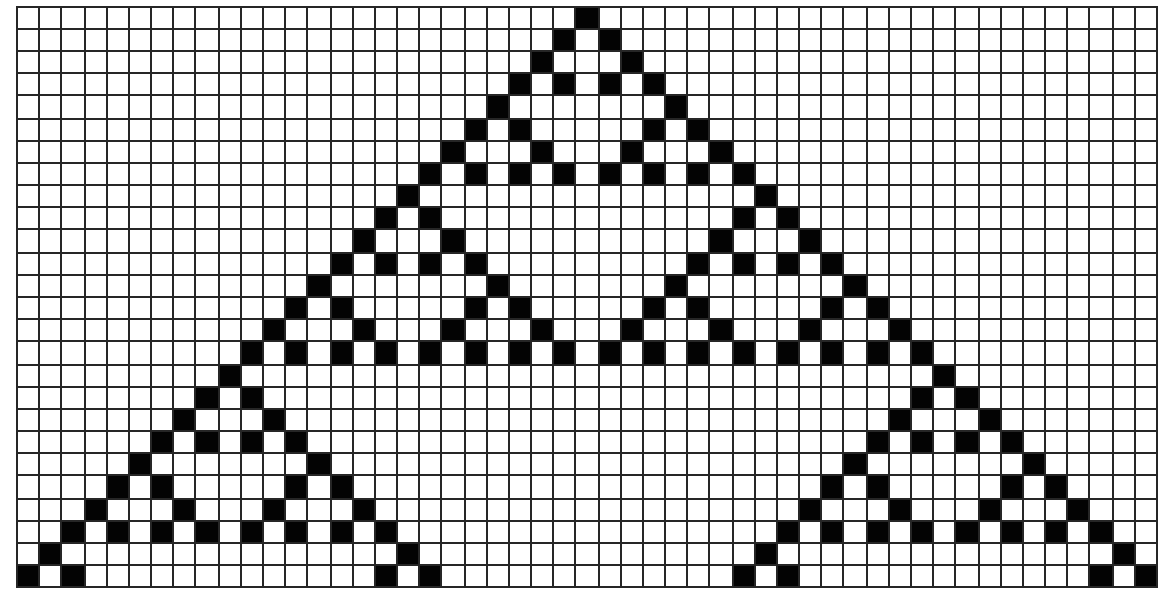
\includegraphics[width=0.75\textwidth]{img/Theory/Cellular_A/Result.png}
    \caption{Sierpiński Triangle, rule 90}
    \label{fig:resultCA}
\end{figure}


In Figure~\ref{fig:resultCA} each line represents an iteration of the system with the application of the rules. With this set of rules a Sierpiński triangle is reproduced.


Cellular automata are used mainly to model phenomena that occur in the physical world, most of them can only express the basic idea of a phenomenon, but some are accurate enough to be able to make predictions.

In this context, cellular automata are used to model natural shapes and textures, the Figure~\ref{fig:CAshell} shows a natural texture on a Textile Cone Snail that looks like the patterns formed with the cellular automaton in the Figure~\ref{fig:CArule30}.



\begin{figure}
        \centering
        \begin{subfigure}[b]{0.3\textwidth}
                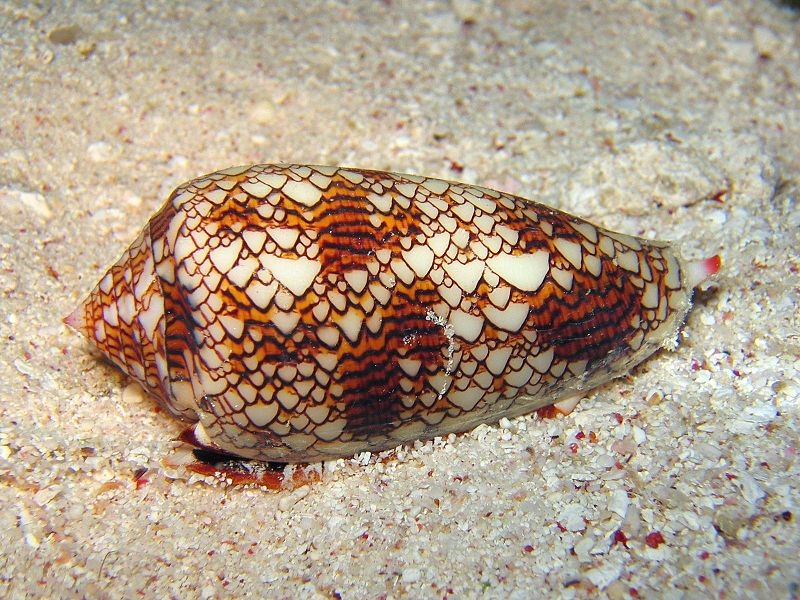
\includegraphics[width=\textwidth]{img/Theory/Cellular_A/shell.jpeg}
                \caption{a)}
				\label{fig:CAshell}
        \end{subfigure}%
        %~ %add desired spacing between images, e. g. ~, \quad, \qquad, \hfill etc.
          %(or a blank line to force the subfigure onto a new line)
          ~~
        \begin{subfigure}[b]{0.5\textwidth}
                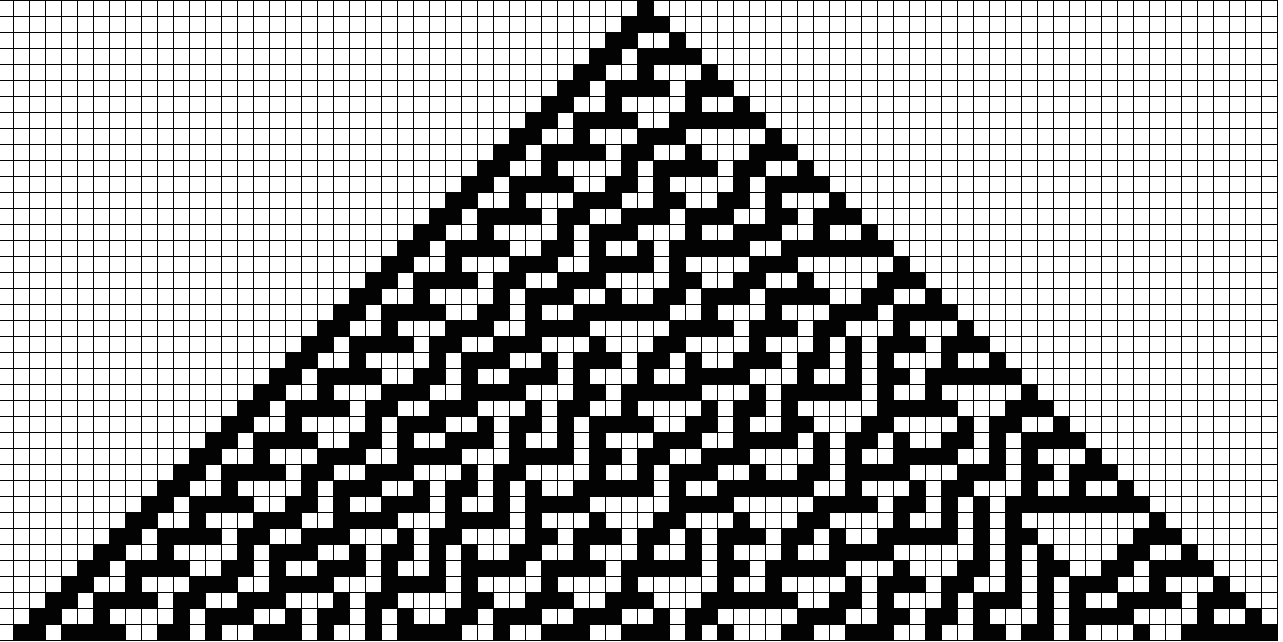
\includegraphics[width=\textwidth]{img/Theory/Cellular_A/Rule30.png}
				\caption{b)}
				\label{fig:CArule30}
        \end{subfigure}
        \caption{Example of the representation of natural patterns with cellular automata. a) Natural Shell, image from \cite{Shiffman2012}. b) Pattern formed with the rule 30.}
		\label{fig:CArule30shell}
\end{figure}



% subsection cellular_automaton (end)

%!TEX root = ../../report.tex

\subsubsection{L-Systems} % (fold)
\label{ssub:l_systems}

Lindenmayer Systems (L-Systems) are a class of string rewriting mechanisms, originally developed by Lindenmayer as a mathematical theory for plant
development. It is capable of describe the behavior of plant cells and model the growth processes of plant development.

An L-Systems consists of two different parts, one axiom and a set of production rules. The axiom is the starting point of the system, acting as a seed. Then it is applied in this seed the set of production rules, that change the initial string, producing other strings.
This is an iterative process, so after the production of a larger set of strings, the rules can be applied to each one of them which grows the size of
the set even more.

L-Systems are used to model the natural growth of vegetation (Figure~\ref{fig:trees}), and the generation of Fractals. 

\begin{figure}[htbp]
    \centering
    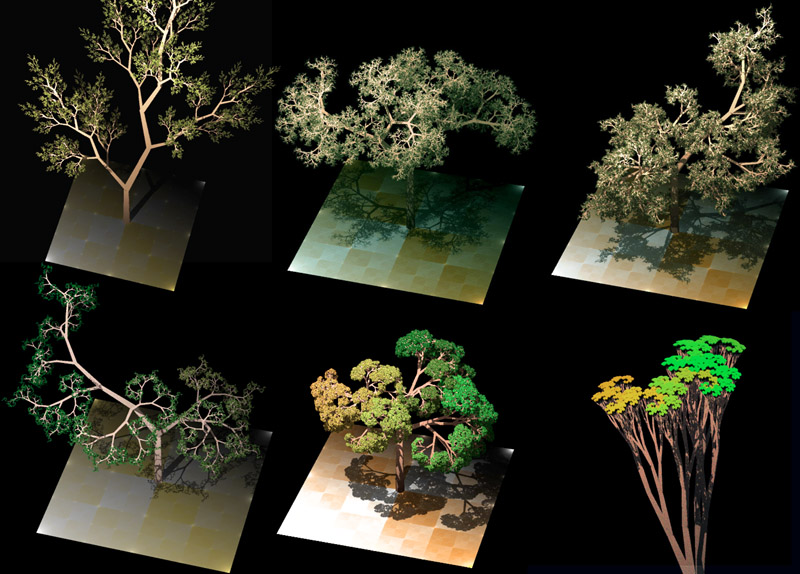
\includegraphics[width=0.65\textwidth]{img/Theory/L_Systems/Dragon_trees.jpg}
    \caption{Trees with L-Systems}
    \label{fig:trees}
\end{figure}


In this process, each symbol is associated with a production rule. For instance having $\{F, +, -\}$ for the alphabet and \emph{production} $\{F \rightarrow
 F+F--F+F\}$. From a starting axiom \emph{aba}, and the application of the rules we have:\\
\begin{equation} \label{eq:seed}
F\\
\end{equation}
\begin{equation} \label{eq:step1}
F+F--F+F\\
\end{equation}
\begin{equation} \label{eq:step2}
F+F--F+F \; + \; F+F--F+F \;- \;- \;F+F--F+F \;+ \;F+F--F+F\\
\end{equation}

%\begin{align}
%\begin{split}
%F\\
%F+F--F+F\\
%F+F--F+F \; + \; F+F--F+F \;- \;- \;F+F--F+F \;+ \;F+F--F+F\\
%\end{split}
%\end{align}
%\\

This is an example of the evolution of one system where the production is applied  in (\ref{eq:seed}) that turns into $F+F--F+F$. Note that the space
between the symbols are just for readability.

All the symbols are assigned with a geometric meaning. The notion of a turtle with a pen, as proposed in \cite{abelson1982aa}, with the symbols being
interpreted as moving instructions to the turtle, is a simple way to understand, where ``F'' means forward and the symbols ``+'' and ``-'' are interpreted as rotations counter-clockwise and clockwise respectively by a predefined angle. By applying this method to the last example and setting the angle for the rotation to $60^{\circ}$ the result is Figure~\ref{fig:kockLS}.

\begin{figure}[htbp]
   \centering
   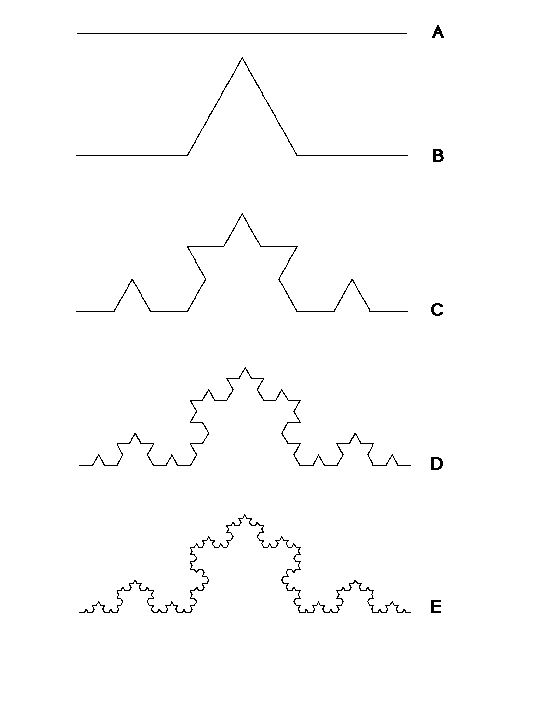
\includegraphics[width=0.55\textwidth]{img/Theory/L_Systems/koch.png}
   \caption{Result of the ``turtle walk'' with the given example}
   \label{fig:kockLS}
\end{figure}

%\begin{wrapfigure}{r}{0.5\textwidth}
%	\vspace{-15pt}
%    \centering
%    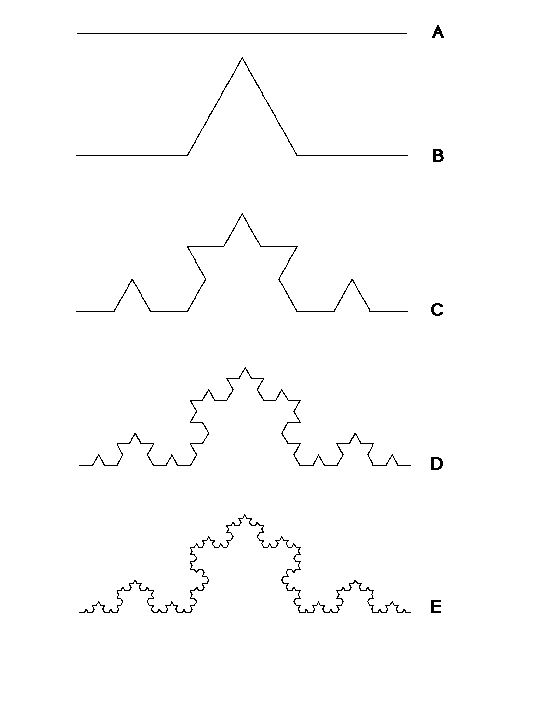
\includegraphics[width=0.55\textwidth]{img/Theory/L_Systems/koch.png}
%    \caption{}
%    \label{fig:kockLS}
%	\vspace{-25pt}
%\end{wrapfigure}

%$\bigodot \; \bigodot$




% This concept of the turtle can be considered also in 3D.



% subsection l_systems (end)

%!TEX root = ../../report.tex

\subsubsection{Shape Grammars} % (fold)
\label{ssub:shape_grammars}


Shape Grammars can be considered grammars for design. In stead of having symbols or letters as components of the alphabet, it has shapes that can be in 2D or 3D. And have production rules that are composed by this shapes, and specify the evolution of the system. With this process, similar to the L-Systems explained before, the shape starts from a seed, i.e. a usually simple shape and can evolve to one big and/or complex shape.

The process is performed in two steps, the recognition of a shape and the replacement according to the rules that are previously defined. 

The Figure~\ref{fig:SGrammars} exemplify one shape grammar, with one rule and the evolution of the application of this rule to the shapes iteratively. In this image, it's shown that from very simple initial shape, can be generated a complex from with a few iterations.

\begin{figure}
        \centering
		\begin{subfigure}[b]{0.7\textwidth}
			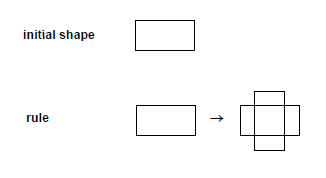
\includegraphics[width=\textwidth]{img/Theory/Shape_Grammars/Grammar.png}
			\caption{a)}
			\label{fig:SGGrammar}
		\end{subfigure}
        
         %add desired spacing between images, e. g. ~, \quad, \qquad, \hfill etc.
          %(or a blank line to force the subfigure onto a new line)
		\begin{subfigure}[b]{0.7\textwidth}
			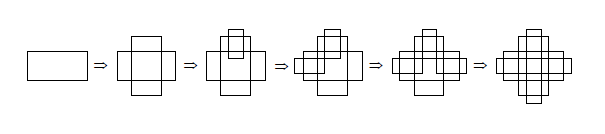
\includegraphics[width=\textwidth]{img/Theory/Shape_Grammars/Recursion.png}
			\caption{b)}
			\label{fig:SGRecursion}
		\end{subfigure}
        \caption{a) Grammar Tiles b) Recursion steps}
        \label{fig:SGrammars}
\end{figure}

This is applied to the generation of buildings in the CityEngine \ref{sub:cityengine} system, using 3D blocks for the main form, and 2D shapes to design the facades.

% \begin{figure}[htbp]
% 	\centering
% 	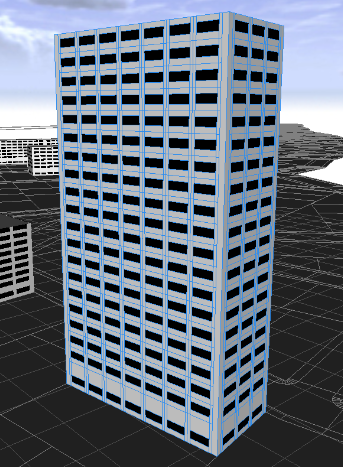
\includegraphics[width=0.55\textwidth]{img/Theory/Shape_Grammars/Edificio.png}
% 	\caption{Simple Building}
% 	\label{fig:SGBuilding}
% \end{figure}

The Figure~\ref{fig:SGBuilding} shows a simple building that I modelled using CityEngine and it's CGA Shape Grammar. But CGA is powerful enough to model much more complex buildings like the Figure~\ref{fig:CEBuilding}.


% \begin{figure}[htbp]
% 	\centering
% 	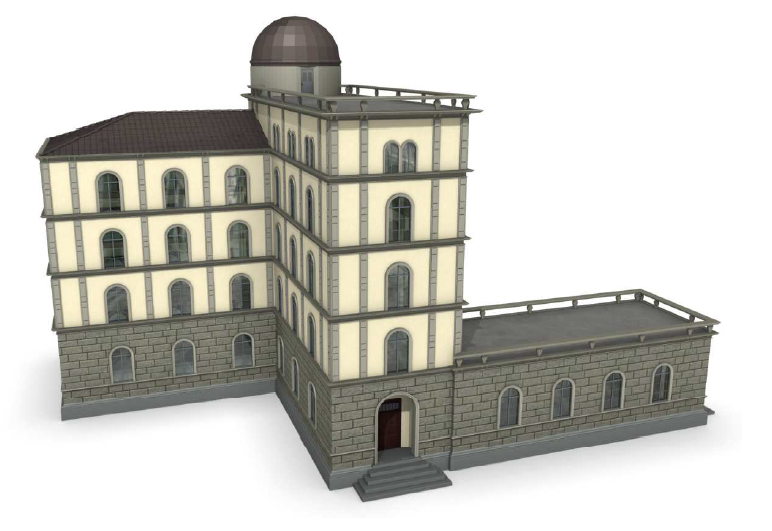
\includegraphics[width=0.55\textwidth]{img/Theory/Shape_Grammars/Capturar.png}
% 	\caption{Complex Building \cite{Muller2006}}
% 	\label{fig:CEBuilding}
% \end{figure}

\begin{figure}
\centering
\begin{minipage}{.5\textwidth}
  \centering
  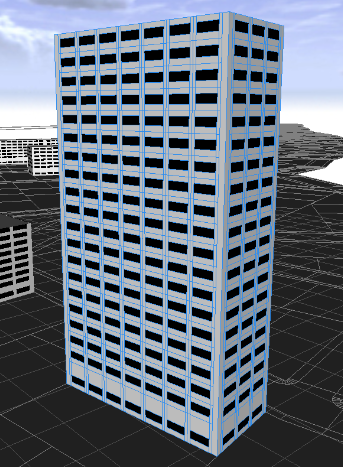
\includegraphics[width=.5\linewidth]{img/Theory/Shape_Grammars/Edificio.png}
  \captionof{figure}{Simple Building}
  \label{fig:SGBuilding}
\end{minipage}%
\begin{minipage}{.5\textwidth}
  \centering
  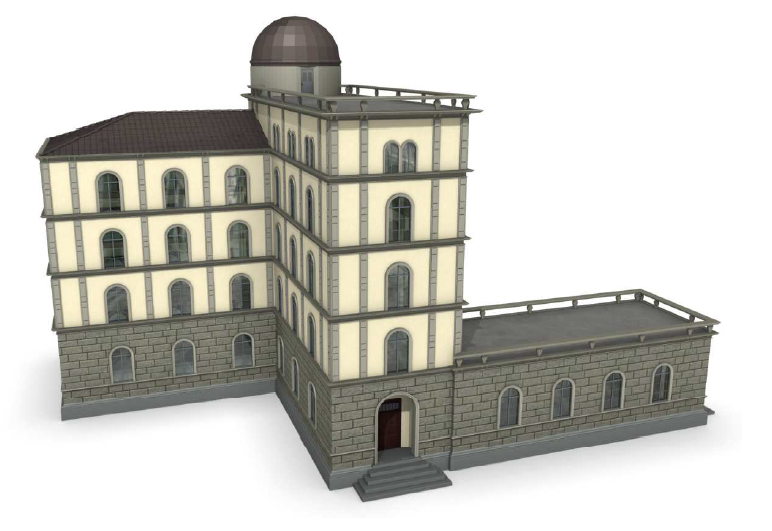
\includegraphics[width=.8\linewidth]{img/Theory/Shape_Grammars/Capturar.png}
  \captionof{figure}{Complex Building \cite{Muller2006}}
  \label{fig:CEBuilding}
\end{minipage}
\end{figure}










% subsubsection shape_grammars (end)

%!TEX root = ../../report.tex

\subsection{Noise} % (fold)
\label{ssub:noise}


``To generate irregular procedural textures, we need an irregular primitive function, usually called noise" \cite{Ebert2002}. It's a pseudorandom function that gave the goal to break the monotony of a pattern and make it look more random.
Perlin Noise is the most known and used noise function. It was created by Ken Perlin, for the movie Tron 1982 with the aiming to generate natural looking textures.

The psedorandom property is important and a true random function like \emph{white noise} would not do the job. If we generate a texture based on white noise the pattern would change every time it's generated and we would like that the it stays the same, frame after frame. This is achieved with the use of inputs for this functions that with the same input returns always the same output sequence. 

The properties of an ideal \emph{noise} functions are as follows \cite{Ebert2002}:
\begin{itemize}
	\item \emph{noise} is a repeatable pseudorandom function of its inputs
	\item \emph{noise} has a known range, namely, from -1 to 1.
	\item \emph{noise} is band-limited, with a maximum frequency of about 1.
	\item \emph{noise} doesn't exhibit obvious periodicities or regular patterns. Such pseudorandom functions are always periodic, but the period can be made very long and therefore the periodicity is not conspicuous.
	\item \emph{noise} is \emph{stationary} - that is, its statistical character should be translationally invariant
	\item \emph{noise} is \emph{isotropic} - that is, its statistical character should be rotationally invariant
\end{itemize}

With this noise function, it's generated a sequence of values that are interpolated to generate a coherent noise. With the application of \emph{turbulence} that is composition of several layers of this noise with different frequencies and amplitudes forming a coherent noise. This layers are called \emph{Octaves} and the ratio between amplitude and frequency of the layers can be expressed as a constant known as \emph{persistence} \cite{Kelly2008}. With the result we can create a texture that looks natural and with fractal like structure.

\begin{figure}[htbp]
	\centering
	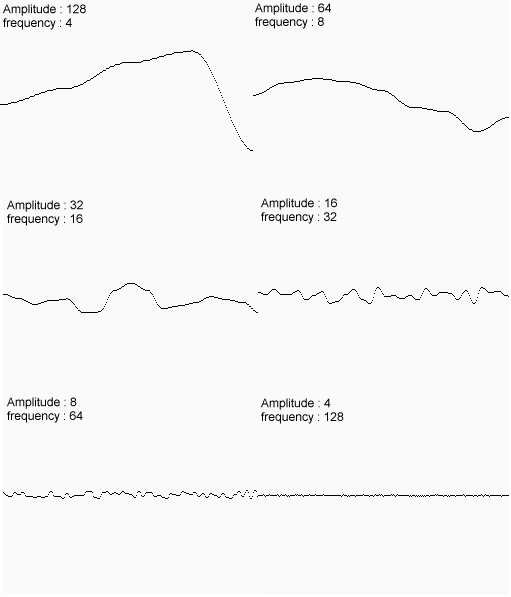
\includegraphics[width=0.55\textwidth]{img/Theory/Perlin_Noise/Merge.png}
	\caption{Different noise functions}
	\label{fig:merge}
\end{figure}

For instance, the Figure~\ref{fig:merge} shows the result of the interpolation over six noise functions with different frequencies and different amplitudes. And the sum of all this functions is the exibithed in the Figure~\ref{fig:noise} \cite{NoisesELIAS}.

\begin{figure}[htbp]
	\centering
	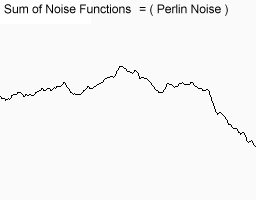
\includegraphics[width=0.55\textwidth]{img/Theory/Perlin_Noise/perlin1.png}
	\caption{``You may even imagine that it looks a little like a mountain range."}
	\label{fig:noise}
\end{figure}

Noise can also be used to generate planes. The method used is the same as the 1D problem but we have to generate a lot more data points that after are interpolated as a plane. This results in noisy images that are often used to model clouds, smoke and other textures with similar visual properties, Figure~\ref{fig:NTextures}. Another application for this technique is the generation of height maps like the one in figure .

\begin{figure}
        \centering
        \begin{subfigure}[b]{0.3\textwidth}
                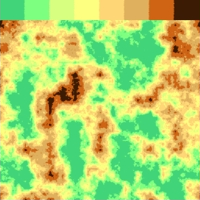
\includegraphics[width=\textwidth]{img/Theory/Perlin_Noise/gradient_discrete.png}
                \label{fig:Fleaf}
        \end{subfigure}%
        ~ %add desired spacing between images, e. g. ~, \quad, \qquad, \hfill etc.
          %(or a blank line to force the subfigure onto a new line)
        \begin{subfigure}[b]{0.3\textwidth}
                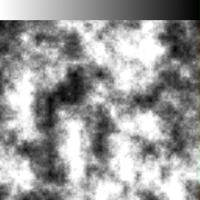
\includegraphics[width=\textwidth]{img/Theory/Perlin_Noise/gradient_grey.png}
                \label{fig:Fbrocoli}
        \end{subfigure}
        ~ %add desired spacing between images, e. g. ~, \quad, \qquad, \hfill etc.
          %(or a blank line to force the subfigure onto a new line)
        \begin{subfigure}[b]{0.3\textwidth}
                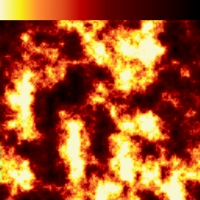
\includegraphics[width=\textwidth]{img/Theory/Perlin_Noise/gradient_fire.png}
                \label{fig:Fbrocoli}
        \end{subfigure}
        \caption{Gradient mapped textures from \cite{NoisesGAMES}}
        \label{fig:NTextures}
\end{figure}

Another application for Noise planes are with \emph{object placement} on a grid. By creating a noise plane with the same size of the grid, with each cell of the grid corresponding to one pixel of noise, the object placement is done by choosing each object for each cell according to the noise value. Figure~\ref{fig:MyNCity}.
Figure~\ref{fig:NCity} shows a city which the buildings where placed with the use of a noise plane. In this case the noise domain was splitted in three intervals, each one corresponds to one type of building (commercial, industrial or residential). After setting the type for one block, the system randomly chooses one from a set of buildings of that type.

\begin{figure}[htbp]
    \centering
    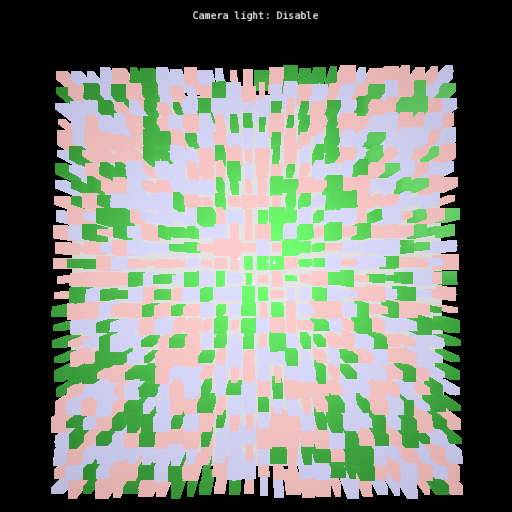
\includegraphics[width=0.55\textwidth]{img/Theory/Perlin_Noise/AppletNoName201501191604.png}
    \caption{Objects Placed following a noise function}
    \label{fig:MyNCity}
\end{figure}

\begin{figure}[htbp]
	\centering
	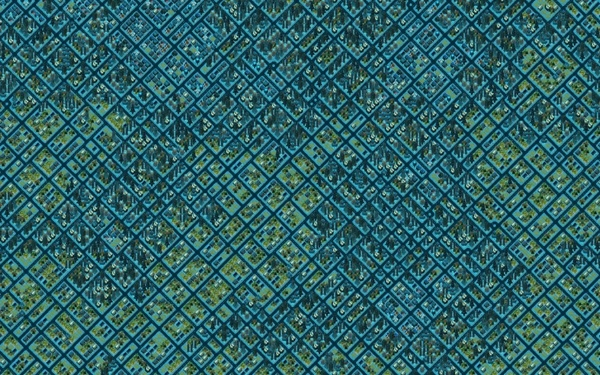
\includegraphics[width=0.55\textwidth]{img/Theory/Perlin_Noise/NoisyCity.jpg}
	\caption{Objects Placed with a noise plane from \cite{NoisesGAMES}}
	\label{fig:NCity}
\end{figure}

% subsubsection noise (end)

%!TEX root = ../../report.tex


\subsection{Other Techniques} % (fold)
\label{sub:other_techniques}

\subsubsection{Level of Detail} % (fold)
\label{ssub:level_of_detail}

Level of Detail (LOD) is a technique that is used to improve the performance of the graphic pipeline. This is done by managing the complexity of the objects representation relative to some indicator.
Within this indicators, the most common one is the distance of each object to the viewer. If an object is far from the viewer a decrease on the detail will not be noticed and will save computation. Other indicators can be the importance that is assigned for each object, relative speed or partial occlusion.

This concept is easy to understand and implement if we look at the example in the Figure~\ref{fig:LOD2}. In this figure there are five cylinders that have different detail according to the distance to the camera. In this case only the number of sides of the cylinder changes.

\begin{figure}[htbp]
	\centering
	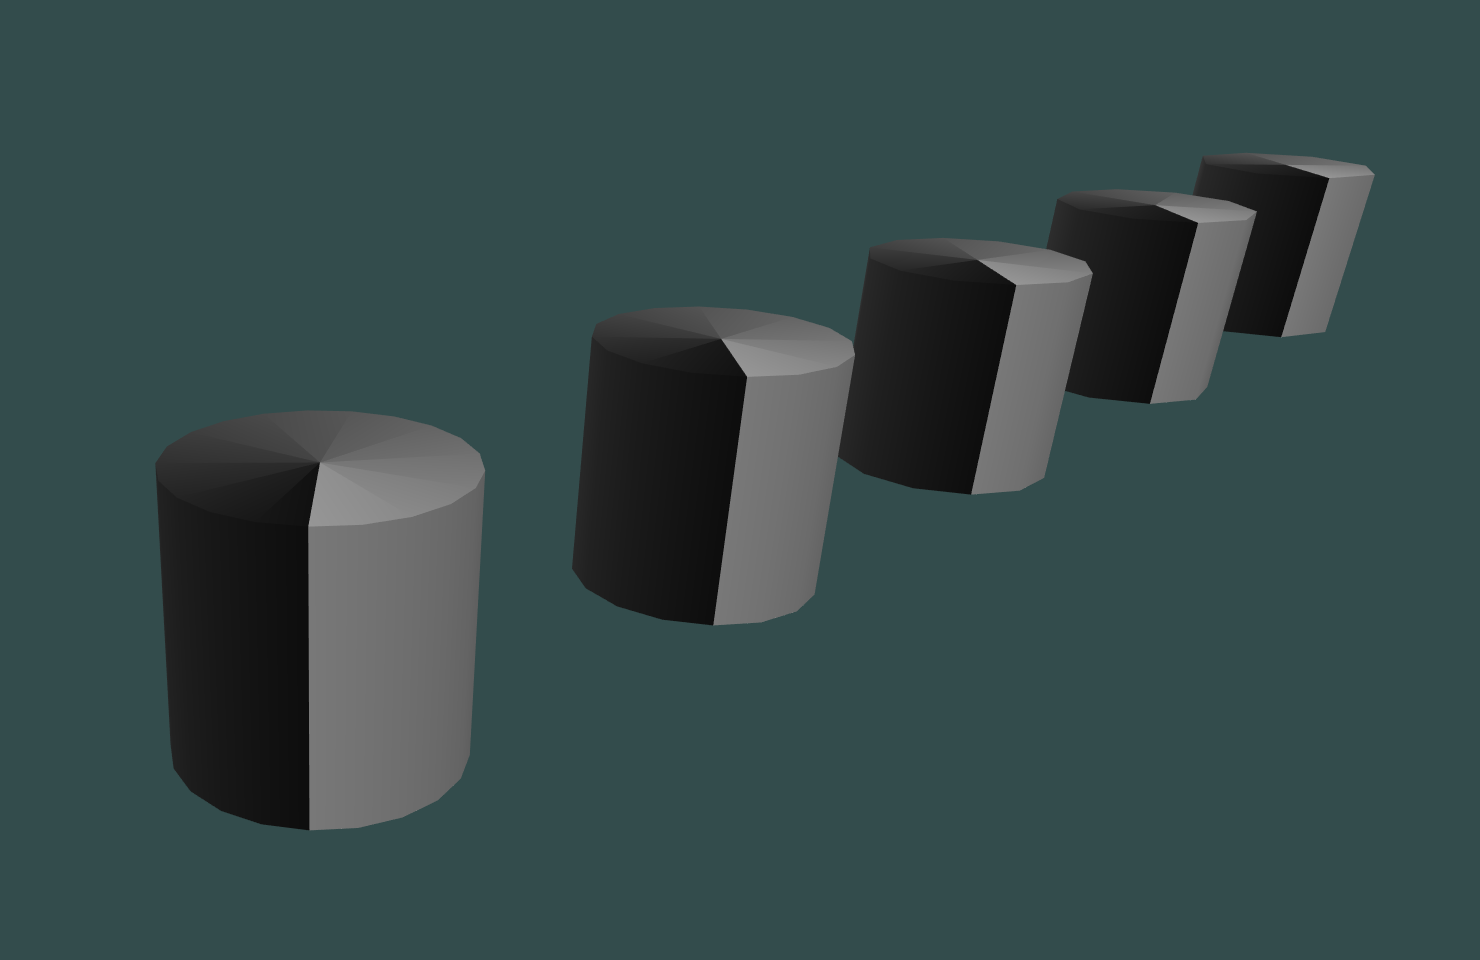
\includegraphics[width=0.95\textwidth]{img/OpenGL/LOD2.png}
	\caption{LOD example}
	\label{fig:LOD2}
\end{figure}
% subsubsection level_of_detail (end)

\subsubsection{Occlusion Culling} % (fold)
\label{ssub:occlusion_culling}

Occlusion culling (OC) is another technique that is used to improve performance. It involves determining the faces that are not visible at each point to be removed from the pipeline.

This procedure is usually done automatically by the GPU and applied to occluded faces behind other objects or out of the viewing frustum.

If this concept is applied before the generation of the objects, and prevent the inclusion of large amounts of geometry through the pipeline, we can make a large improvement on performance. The Figure~\ref{fig:viewingRange} is a good example. Here only the buildings that are visible from the current point are generated.

% subsubsection occlusion_culling (end)


% subsection other_techniques (end)

%!TEX root = ../../report.tex

\subsection{Modern OpenGL} % (fold)
\label{sub:modern_opengl}

Majors changes has been imposed to this library from it's early versions and this section covers the modern version of OpenGL, after version 3.2.

OpenGL is an well known cross-platform Application Programming Interface (API) created by Silicon Graphics Computer Systems with Version 1.0 released in July of 1994 for 3-D Graphics and Imaging. It's a streamlined and hardware-independent interface that can be implemented on manny different types of graphics hardware. It's also independent of the machine's operative and windowing systems.

OpenGL provides a small set of geometric primitives - points, lines, triangles and patches that are specified by their vertices. And from this geometric primitives all geometry is constructed, both in 2D and 3D. 

Shaders ``are special functions that the graphics hardware executes. The best way to think of shaders is as little programs that are specifically compiled for your graphics processing unit''. \cite{shreiner2013opengl}

There are some steps that are performed to render an image. First the model is created from geometric primitives and this data is the input  for the pipline(Vertex Data) in Figure~\ref{fig:OGLPipeline}. 

\begin{figure}[htbp]
	\centering
	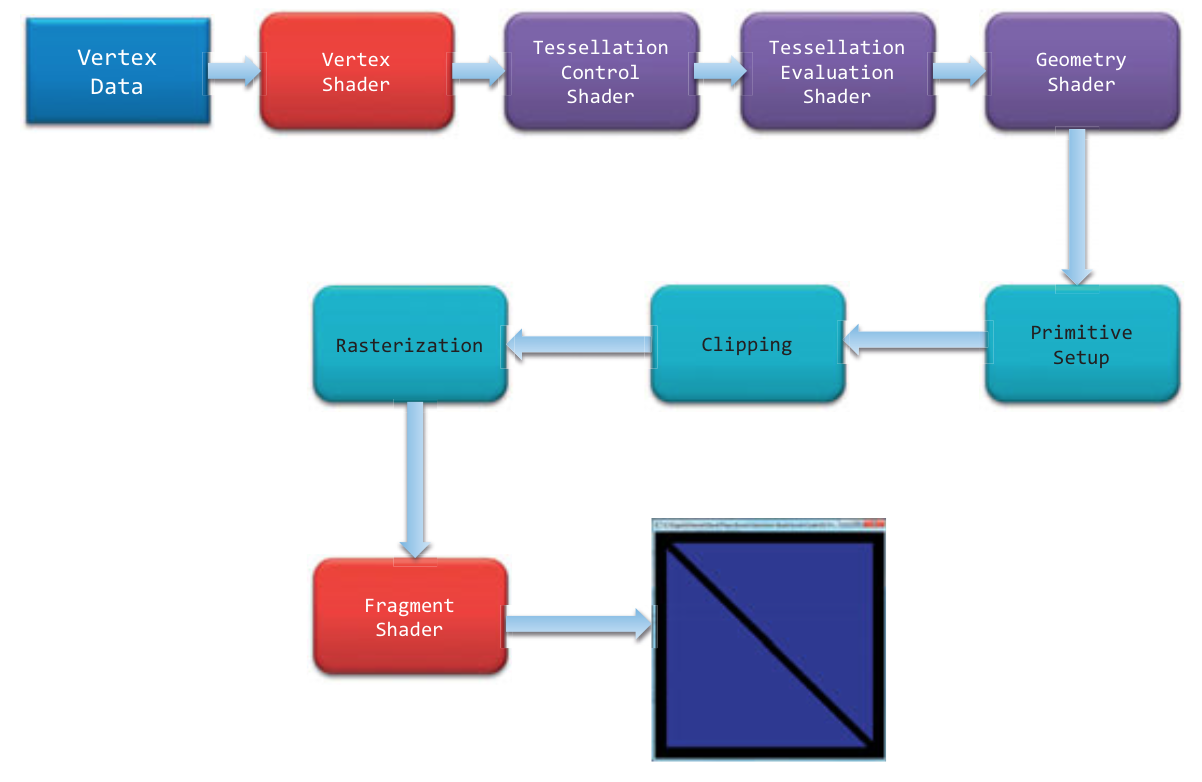
\includegraphics[width=0.95\textwidth]{img/OpenGL/pipeline.png}
	\caption{OpenGL Pipeline \cite{shreiner2013opengl}}
	\label{fig:OGLPipeline}
\end{figure}


The first step of the pipeline is the Vertex Shader that process the data associated with each vertex. 

After this, there are three optional shaders. In this three there are two Tesselation Shaders. With this shaders simple geometries can be tesselated and increase of the number of primitives to improve the models dynamically.

The third optional shader is the Geometric Shader that allows the aditional processing of geometric primitives and also including the creation of new primitives.

Until now all steps work with vertices, and after those steps there are three fixed steps, primitive assembly, clipping and rasterization that assembly the vertices into primitives, clip the geometry cutting the parts that falls of the ``screen'' and the generation of fragments respectively.

A fragments is a ``‘candidate pixel’, in that pixels have a home in the framebuffer, while a fragment still can be rejected and never update its associated pixel location'' \cite{shreiner2013opengl}.
\subsection{Vertex Shaders} % (fold)
\label{sub:vertex_shaders}
Vertex Shaders can be very simple, from a \emph{pass-through shader} that just copies the data to the next step to very complex ones.

In this shaders are used to performed computations to calculate the position of the vertices in screen coordinates, assign vertex's color using lightning computations, etc..

Vertex Shaders have some limitations, they cannot create additional geometry and cannot access data of other vertices. They can just process the data of the current vertex and the number of vertices after this step is the same as before.

% subsection vertex_shaders (end)

\subsection{Tesselation Shaders} % (fold)
\label{sub:tesselation_shaders}
Tesselation Shaders are very different form the previous ones. This shaders address some of limitations presented before.
This shaders work with a geometric primitive called a \emph{patch}.

\subsubsection{Patch} % (fold)
\label{ssub:patch}
	Are lists of vertices that preserves their order during processing. This is because each patch can have an arbitrary number of vertices that have to be specified before drawing oposing to the other primitives that have a specific/pre-assigned/fixed number of vertices.
% subsubsection patch (end)

\subsubsection{Tesselation Control Shader} % (fold)
\label{ssub:tesselation_control_shader}
	This shader generates the tesselation output-patch vertices and specify the tesselation level factors. 

	The output-patch vertices are the list of vertices that results after the input vertices have been processed. 

	The tesselation level factor defines how much the output patch is tesselated. 

	OpenGL supports three tesselation domains: a quadrilateral, a triangle, and a collection of isolines \cite{shreiner2013opengl}. To control the amount of tesselation two sets of values are set, the outer-tesselation values and the inner-tesselation values. This values define how the perimeter or the interior of the domain are subdivided respectivelly.

% subsubsection tesselation_control_shader (end)

\subsubsection{Tesselation Evaluation Shaders} % (fold)
\label{ssub:tesselation_evaluation_shaders}
Tesselation shaders work with the output of the previous phase. Here the vertex positions are calculated from the tessellation computed before. It's is basically responsible for the caclulation of the vertices screen positions from the layout defined.

% subsubsection tesselation_evaluation_shaders (end)

% subsection tesselation_shaders (end)

\subsection{Geometric Shaders} % (fold)
\label{sub:geometric_shaders}

Geometry Shaders are the first shaders that access the complete primitive as a list of vertices and with that it's allowed to do different actions that require this access to information. The amount of output can be variable so both \emph{culling geometry} and \emph{geometry amplification}, respectivelly output less vertices that the input and output more vertices than the input. Also in this shaders the primitives type can be modified, i. e. the input can be \emph{quads} and the output be a \emph{triangle\_strip}.

% subsection geometric_shaders (end)

\subsection{Fragment Shaders} % (fold)
\label{sub:fragment_shaders}
This shaders implement the last phase of the pipeline. Here the fragment's final color is computed and also the depth value.

Fragment Shaders are usefull to implement texture mapping or lights for instance.

% subsection fragment_shaders (end)
% subsection modern_opengl (end)

